\subsection{Kernel configuration}

\begin{frame}
  \frametitle{Kernel configuration and build system}
  \begin{itemize}
  \item The kernel configuration and build system is based on multiple
    Makefiles
  \item One only interacts with the main \code{Makefile}, present at
    the {\bf top directory} of the kernel source tree
  \item Interaction takes place
    \begin{itemize}
    \item using the \code{make} tool, which parses the Makefile
    \item through various {\bf targets}, defining which action should
      be done (configuration, compilation, installation, etc.). Run
      \code{make help} to see all available targets.
    \end{itemize}
  \item Example
    \begin{itemize}
    \item \code{cd linux-3.6.x/}
    \item \code{make <target>}
    \end{itemize}
  \end{itemize}
\end{frame}

\begin{frame}
  \frametitle{Kernel configuration (1)}
  \begin{itemize}
  \item The kernel contains thousands of device drivers, filesystem
    drivers, network protocols and other configurable items
  \item Thousands of options are available, that are used to
    selectively compile parts of the kernel source code
  \item The kernel configuration is the process of defining the set of
    options with which you want your kernel to be compiled
  \item The set of options depends
    \begin{itemize}
    \item On your hardware (for device drivers, etc.)
    \item On the capabilities you would like to give to your kernel
      (network capabilities, filesystems, real-time, etc.)
    \end{itemize}
  \end{itemize}
\end{frame}

\begin{frame}
  \frametitle{Kernel configuration (2)}
  \begin{itemize}
  \item The configuration is stored in the \code{.config} file at the
    root of kernel sources
    \begin{itemize}
    \item Simple text file, \code{key=value} style
    \end{itemize}
  \item As options have dependencies, typically never edited by hand,
    but through graphical or text interfaces:
    \begin{itemize}
    \item \code{make xconfig}, \code{make gconfig} (graphical)
    \item \code{make menuconfig}, \code{make nconfig} (text)
    \item You can switch from one to another, they all load/save the
      same \code{.config} file, and show the same set of options
    \end{itemize}
  \item To modify a kernel in a GNU/Linux distribution: the
    configuration files are usually released in \code{/boot/},
    together with kernel images: \code{/boot/config-3.2.0-31-generic}
  \end{itemize}
\end{frame}

\begin{frame}
  \frametitle{Kernel or module?}
  \begin{itemize}
  \item The {\bf kernel image} is a {\bf single file}, resulting from
    the linking of all object files that correspond to features
    enabled in the configuration
    \begin{itemize}
    \item This is the file that gets loaded in memory by the
      bootloader
    \item All included features are therefore available as soon as the
      kernel starts, at a time where no filesystem exists
    \end{itemize}
  \item Some features (device drivers, filesystems, etc.) can however
    be compiled as {\bf modules}
    \begin{itemize}
    \item Those are {\em plugins} that can be loaded/unloaded dynamically to
      add/remove features to the kernel
    \item Each {\bf module is stored as a separate file in the
        filesystem}, and therefore access to a filesystem is mandatory
      to use modules
    \item This is not possible in the early boot procedure of the
      kernel, because no filesystem is available
    \end{itemize}
  \end{itemize}
\end{frame}

\begin{frame}
  \frametitle{Kernel option types}
  \begin{itemize}
  \item There are different types of options
    \begin{itemize}
    \item \code{bool} options, they are either
      \begin{itemize}
      \item {\em true} (to include the feature in the kernel) or
      \item {\em false} (to exclude the feature from the kernel)
      \end{itemize}
    \item \code{tristate} options, they are either
      \begin{itemize}
      \item {\em true} (to include the feature in the kernel image) or
      \item {\em module} (to include the feature as a kernel module) or
      \item {\em false} (to exclude the feature)
      \end{itemize}
    \item \code{int} options, to specify integer values
    \item \code{string} options, to specify string values
    \end{itemize}
  \end{itemize}
\end{frame}

\begin{frame}
  \frametitle{Kernel option dependencies}
  \begin{itemize}
  \item There are dependencies between kernel options
  \item For example, enabling a network driver requires the network
    stack to be enabled
  \item Two types of dependencies
    \begin{itemize}
    \item \code{depends on} dependencies. In this case, option A that
      depends on option B is not visible until option B is enabled
    \item \code{select} dependencies. In this case, with option A
      depending on option B, when option A is enabled, option B is
      automatically enabled
    \item \code{make xconfig} allows to see all options, even those
      that cannot be selected because of missing dependencies. In this
      case, they are displayed in gray
    \end{itemize}
  \end{itemize}
\end{frame}

\begin{frame}
  \frametitle{make xconfig}
  \code{make xconfig}
  \begin{itemize}
  \item The most common graphical interface to configure the kernel.
  \item Make sure you read\\
    \code{help ->  introduction: useful options!}
  \item File browser: easier to load configuration files
  \item Search interface to look for parameters
  \item Required Debian / Ubuntu packages: \code{libqt4-dev} \code{g++}
    (\code{libqt3-mt-dev} for older kernel releases)
  \end{itemize}
\end{frame}

\begin{frame}
  \frametitle{make xconfig screenshot}
  \begin{center}
    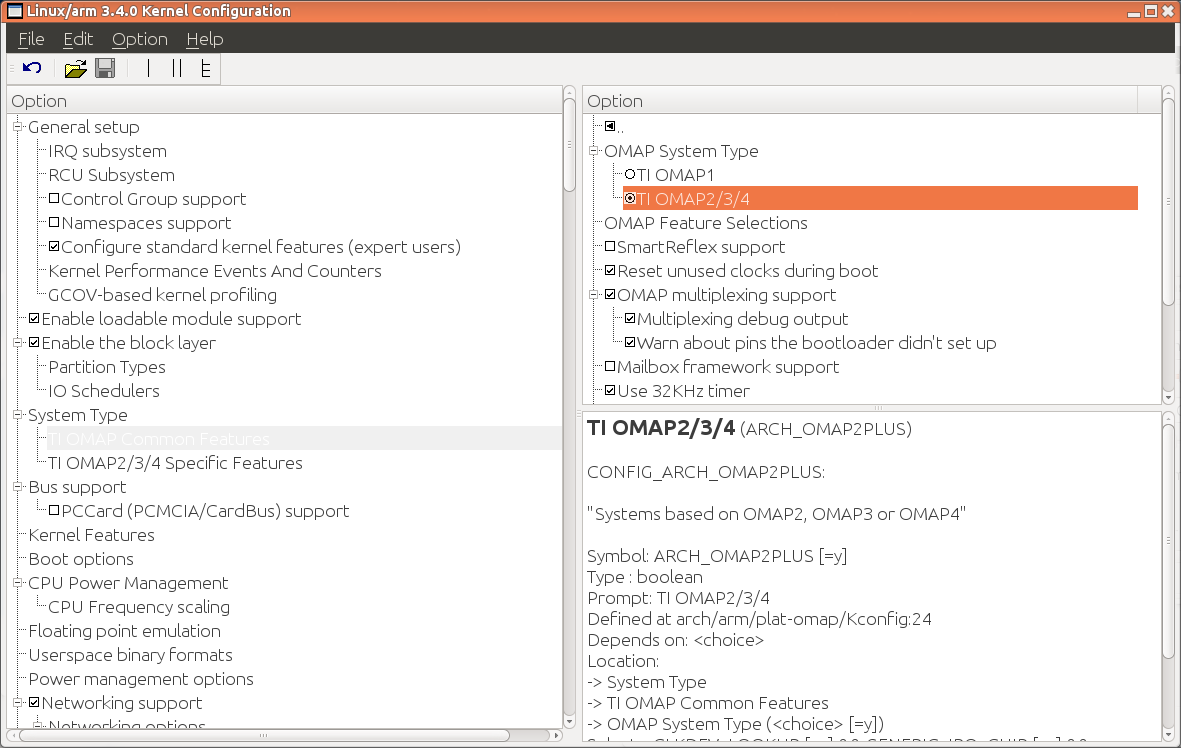
\includegraphics[width=\textwidth]{slides/sysdev-linux-intro-configuration/xconfig-screenshot.png}
  \end{center}
\end{frame}

\begin{frame}
  \frametitle{make xconfig search interface}

  Looks for a keyword in the parameter name. Allows to select or
  unselect found parameters.

  \begin{center}
    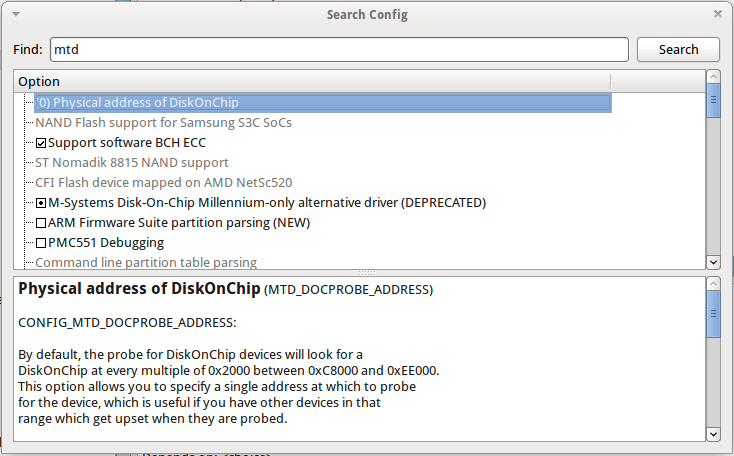
\includegraphics[width=0.9\textwidth]{slides/sysdev-linux-intro-configuration/xconfig-search.png}
  \end{center}
\end{frame}

\begin{frame}
\frametitle{Kernel configuration options}
  \begin{center}
    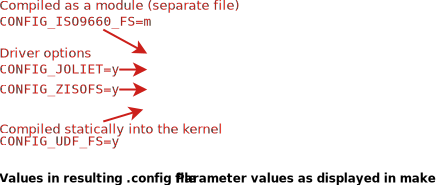
\includegraphics[width=\textwidth]{slides/sysdev-linux-intro-configuration/xconfig-iso-example.pdf}
  \end{center}
\end{frame}

\begin{frame}[fragile]
  \frametitle{Corresponding .config file excerpt}
  Options are grouped by sections and are prefixed with
  \code{CONFIG_}.
\small
\begin{verbatim}
#
# CD-ROM/DVD Filesystems
#
CONFIG_ISO9660_FS=m
CONFIG_JOLIET=y
CONFIG_ZISOFS=y
CONFIG_UDF_FS=y
CONFIG_UDF_NLS=y

#
# DOS/FAT/NT Filesystems
#
# CONFIG_MSDOS_FS is not set
# CONFIG_VFAT_FS is not set
CONFIG_NTFS_FS=m
# CONFIG_NTFS_DEBUG is not set
CONFIG_NTFS_RW=y
\end{verbatim}
\end{frame}

\begin{frame}
  \frametitle{make gconfig}
  \begin{columns}
    \column{0.5\textwidth}
    \code{make gconfig}
    \begin{itemize}
      \item {\em GTK} based graphical configuration interface. Functionality
            similar to that of make \code{xconfig}.
      \item Just lacking a search functionality.
      \item Required Debian packages: \code{libglade2-dev}
    \end{itemize}
    \column{0.5\textwidth}
    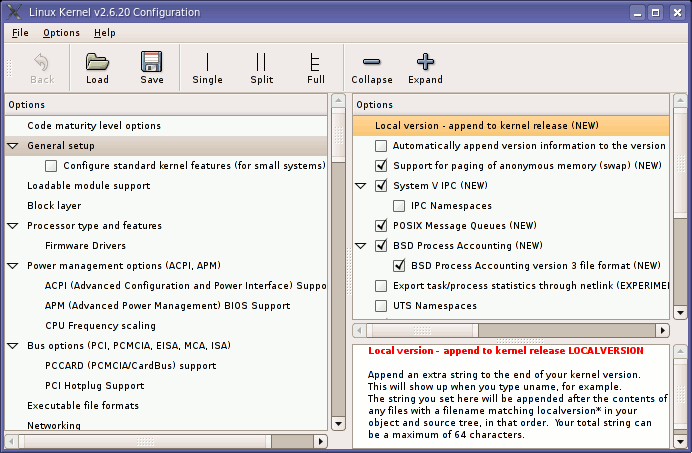
\includegraphics[width=0.9\textwidth]{slides/sysdev-linux-intro-configuration/gconfig-screenshot.png}
  \end{columns}
\end{frame}

\begin{frame}
  \frametitle{make menuconfig}
  \begin{columns}
    \column{0.5\textwidth}
    \code{make menuconfig}
    \begin{itemize}
      \item Useful when no graphics are available. Pretty convenient too!
      \item Same interface found in other tools: BusyBox, Buildroot...
      \item Required Debian packages: \code{libncurses-dev}
    \end{itemize}
    \column{0.5\textwidth}
    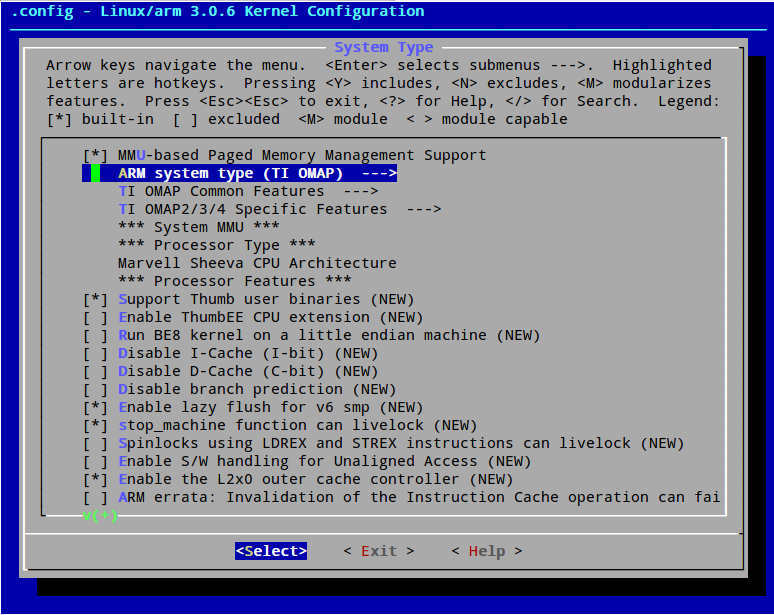
\includegraphics[width=0.9\textwidth]{slides/sysdev-linux-intro-configuration/menuconfig-screenshot.png}
  \end{columns}
\end{frame}

\begin{frame}
  \frametitle{make nconfig}
  \begin{columns}
    \column{0.5\textwidth}
    \code{make nconfig}
    \begin{itemize}
      \item A newer, similar text interface
      \item More user friendly (for example, easier to access help information).
      \item Required Debian packages: \code{libncurses-dev}
    \end{itemize}
    \column{0.5\textwidth}
    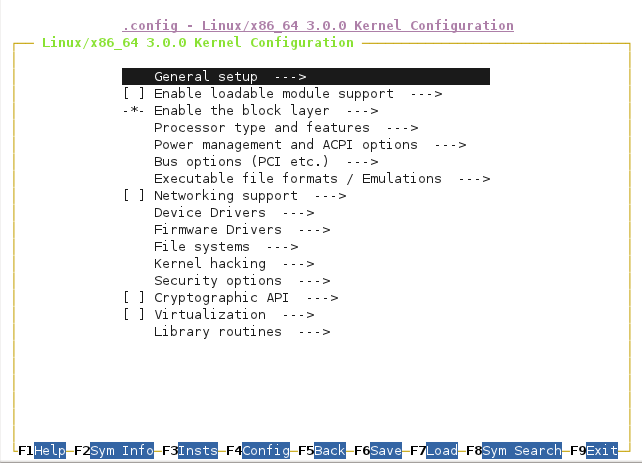
\includegraphics[width=0.9\textwidth]{slides/sysdev-linux-intro-configuration/nconfig-screenshot.png}
  \end{columns}
\end{frame}

\begin{frame}
  \frametitle{make oldconfig}
  \code{make oldconfig}
  \begin{itemize}
  \item Needed very often!
  \item Useful to upgrade a \code{.config} file from an earlier kernel release
  \item Issues warnings for configuration parameters that no longer
    exist in the new kernel.
  \item Asks for values for new parameters
  \end{itemize}
  If you edit a \code{.config} file by hand, it's strongly recommended
  to run \code{make oldconfig} afterwards!
\end{frame}

\begin{frame}
  \frametitle{make allnoconfig}
  \code{make allnoconfig}
  \begin{itemize}
  \item Only sets strongly recommended settings to \code{y}.
  \item Sets all other settings to \code{n}.
  \item Very useful in embedded systems to select only the minimum
    required set of features and drivers.
  \item Much more convenient than unselecting hundreds of features one
    by one!
  \end{itemize}
\end{frame}

\begin{frame}
  \frametitle{Undoing configuration changes}
  A frequent problem:
  \begin{itemize}
  \item After changing several kernel configuration settings, your
    kernel no longer works.
  \item If you don't remember all the changes you made,
    you can get back to your previous configuration:\\
    \code{$ cp .config.old .config}
  \item All the configuration interfaces of the kernel
    (\code{xconfig}, \code{menuconfig}, \code{allnoconfig}...) keep
    this \code{.config.old} backup copy.
  \end{itemize}
\end{frame}

\begin{frame}
  \frametitle{Configuration per architecture}
  \begin{itemize}
  \item The set of configuration options is architecture dependent
    \begin{itemize}
    \item Some configuration options are very architecture-specific
    \item Most of the configuration options (global kernel options,
      network subsystem, filesystems, most of the device drivers) are
      visible in all architectures.
    \end{itemize}
  \item By default, the kernel build system assumes that the kernel is
    being built for the host architecture, i.e. native compilation
  \item The architecture is not defined inside the configuration, but
    at a higher level
  \item We will see later how to override this behaviour, to allow the
    configuration of kernels for a different architecture
  \end{itemize}
\end{frame}

\begin{frame}
  \frametitle{Overview of kernel options (1)}
  \begin{itemize}
  \item General setup
    \begin{itemize}
    \item {\em Local version - append to kernel release} allows to
      concatenate an arbitrary string to the kernel version that a
      user can get using \code{uname -r}. Very useful for support!
    \item {\em Support for swap}, can usually be disabled on most
      embedded devices
    \item {\em Configure standard kernel features (expert users)}
      allows to remove features from the kernel to reduce its
      size. Powerful, but use with care!
    \end{itemize}
  \end{itemize}
\end{frame}

\begin{frame}
  \frametitle{Overview of kernel options (2)}
  \begin{itemize}
  \item Loadable module support
    \begin{itemize}
    \item Allows to enable or completely disable module support. If
      your system doesn't need kernel modules, best to disable since
      it saves a significant amount of space and memory
    \end{itemize}
  \item Enable the block layer
    \begin{itemize}
    \item If \code{CONFIG_EXPERT} is enabled, the block layer can be
      completely removed. Embedded systems using only flash storage
      can safely disable the block layer
    \end{itemize}
  \item Processor type and features (x86) or System type (ARM) or CPU selection
    (MIPS)
    \begin{itemize}
    \item Allows to select the CPU or machine for which the kernel
      must be compiled
    \item On x86, only optimization-related, on other architectures
      very important since there's no compatibility
    \end{itemize}
  \end{itemize}
\end{frame}

\begin{frame}
  \frametitle{Overview of kernel options (3)}
  \begin{itemize}
  \item Kernel features
    \begin{itemize}
    \item Tickless system, which allows to disable the regular timer
      tick and use on-demand ticks instead. Improves power savings
    \item High resolution timer support. By default, the resolution of
      timer is the tick resolution. With high resolution timers, the
      resolution is as precise as the hardware can give
    \item Preemptible kernel enables the preemption inside the kernel
      code (the userspace code is always preemptible). See our
      real-time presentation for details
    \end{itemize}
  \item Power management
    \begin{itemize}
    \item Global power management option needed for all power
      management related features
    \item Suspend to RAM, CPU frequency scaling, CPU idle control,
      suspend to disk
    \end{itemize}
  \end{itemize}
\end{frame}

\begin{frame}
  \frametitle{Overview of kernel options (4)}
  \begin{itemize}
  \item Networking support
    \begin{itemize}
    \item The network stack
    \item Networking options
      \begin{itemize}
      \item Unix sockets, needed for a form of inter-process
        communication
      \item TCP/IP protocol with options for multicast, routing,
        tunneling, Ipsec, Ipv6, congestion algorithms, etc.
      \item Other protocols such as DCCP, SCTP, TIPC, ATM
      \item Ethernet bridging, QoS, etc.
      \end{itemize}
    \item Support for other types of network
      \begin{itemize}
      \item CAN bus, Infrared, Bluetooth, Wireless stack, WiMax stack,
        etc.
      \end{itemize}
    \end{itemize}
  \end{itemize}
\end{frame}

\begin{frame}
  \frametitle{Overview of kernel options (5)}
  \begin{itemize}
  \item Device drivers
    \begin{itemize}
    \item MTD is the subsystem for flash (NOR, NAND, OneNand,
      battery-backed memory, etc.)
    \item Parallel port support
    \item Block devices, a few misc block drivers such as loopback,
      NBD, etc.
    \item ATA/ATAPI, support for IDE disk, CD-ROM and tapes. A new
      stack exists
    \item SCSI
      \begin{itemize}
      \item The SCSI core, needed not only for SCSI devices but also
        for USB mass storage devices, SATA and PATA hard drives, etc.
      \item SCSI controller drivers
      \end{itemize}
    \end{itemize}
  \end{itemize}
\end{frame}

\begin{frame}
  \frametitle{Overview of kernel options (6)}
  \begin{itemize}
  \item Device drivers (cont)
    \begin{itemize}
    \item SATA and PATA, the new stack for hard disks, relies on SCSI
    \item RAID and LVM, to aggregate hard drivers and do replication
    \item Network device support, with the network controller
      drivers. Ethernet, Wireless but also PPP
    \item Input device support, for all types of input devices:
      keyboards, mice, joysticks, touchscreens, tablets, etc.
    \item Character devices, contains various device drivers, amongst
      them
      \begin{itemize}
      \item serial port controller drivers
      \item PTY driver, needed for things like SSH or telnet
      \end{itemize}
    \item I2C, SPI, 1-wire, support for the popular embedded buses
    \item Hardware monitoring support, infrastructure and drivers for
      thermal sensors
    \end{itemize}
  \end{itemize}
\end{frame}

\begin{frame}
  \frametitle{Overview of kernel options (7)}
  \begin{itemize}
  \item Device drivers (cont)
    \begin{itemize}
    \item Watchdog support
    \item Multifunction drivers are drivers that do not fit in any
      other category because the device offers multiple functionality
      at the same time
    \item Multimedia support, contains the V4L and DVB subsystems, for
      video capture, webcams, AM/FM cards, DVB adapters
    \item Graphics support, infrastructure and drivers for
      framebuffers
    \item Sound card support, the OSS and ALSA sound infrastructures
      and the corresponding drivers
    \item HID devices, support for the devices that conform to the HID
      specification (Human Input Devices)
    \end{itemize}
  \end{itemize}
\end{frame}

\begin{frame}
  \frametitle{Overview of kernel options (8)}
  \begin{itemize}
  \item Device drivers (cont)
    \begin{itemize}
    \item USB support
      \begin{itemize}
      \item Infrastructure
      \item Host controller drivers
      \item Device drivers, for devices connected to the embedded system
      \item Gadget controller drivers
      \item Gadget drivers, to let the embedded system act as a
        mass-storage device, a serial port or an Ethernet adapter
      \end{itemize}
    \item MMC/SD/SDIO support
    \item LED support
    \item Real Time Clock drivers
    \item Voltage and current regulators
    \item Staging drivers, crappy drivers being cleaned up
    \end{itemize}
  \end{itemize}
\end{frame}

\begin{frame}
  \frametitle{Overview of kernel options (9)}
  \begin{itemize}
  \item For some categories of devices the driver is not implemented
    inside the kernel
    \begin{itemize}
    \item Printers
    \item Scanners
    \item Graphics drivers used by X.org
    \item Some USB devices
    \end{itemize}
  \item For these devices, the kernel only provides a mechanism to
    access the hardware, the driver is implemented in userspace
  \end{itemize}
\end{frame}

\begin{frame}
  \frametitle{Overview of kernel options (10)}
  \begin{itemize}
  \item File systems
    \begin{itemize}
    \item The common Linux filesystems for block devices: ext2, ext3,
      ext4
    \item Less common filesystems: XFS, JFS, ReiserFS, GFS2, OCFS2,
      Btrfs
    \item CD-ROM filesystems: ISO9660, UDF
    \item DOS/Windows filesystems: FAT and NTFS
    \item Pseudo filesystems: proc and sysfs
    \item Miscellaneous filesystems, with amongst other flash
      filesystems such as JFFS2, UBIFS, SquashFS, cramfs
    \item Network filesystems, with mainly NFS and SMB/CIFS
    \end{itemize}
  \item Kernel hacking
    \begin{itemize}
    \item Debugging features useful for kernel developers
    \end{itemize}
  \end{itemize}
\end{frame}
